% ------------------------------------------------------------------------------
\clearpage
\section{Multivariate Analysis}
% ------------------------------------------------------------------------------

\begin{figure}[htbp]
  \centering

  \begin{subfigure}[t]{.49\textwidth}
    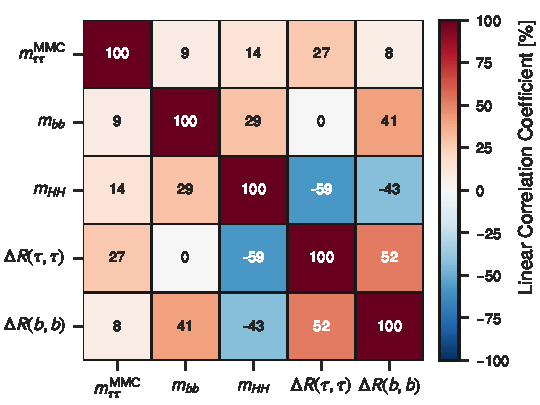
\includegraphics[width=\textwidth]{mva/correlations/NonResHH_pearson}
    \subcaption{SM \HH (gluon fusion)}
  \end{subfigure}\hfill %
  \begin{subfigure}[t]{.49\textwidth}
    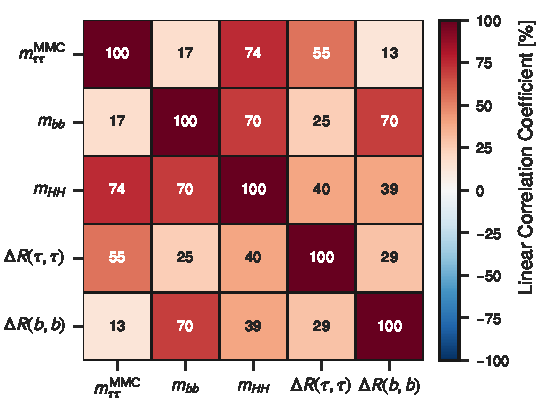
\includegraphics[width=\textwidth]{mva/correlations/ttbar_pearson}
    \subcaption{\ttbar}
  \end{subfigure}

  \begin{subfigure}[t]{.49\textwidth}
    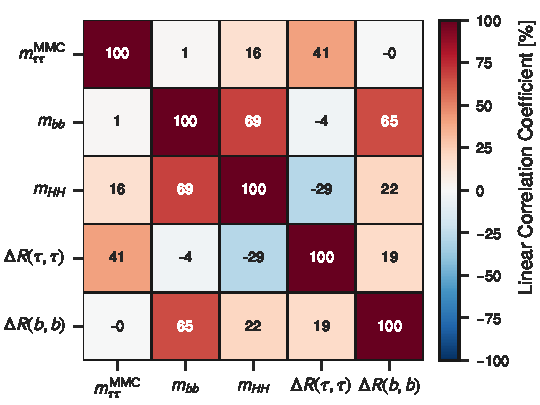
\includegraphics[width=\textwidth]{mva/correlations/Ztautau_pearson}
    \subcaption{$Z \rightarrow \tautau + \text{jets}$}
  \end{subfigure}\hfill %
  \begin{subfigure}[t]{.49\textwidth}
    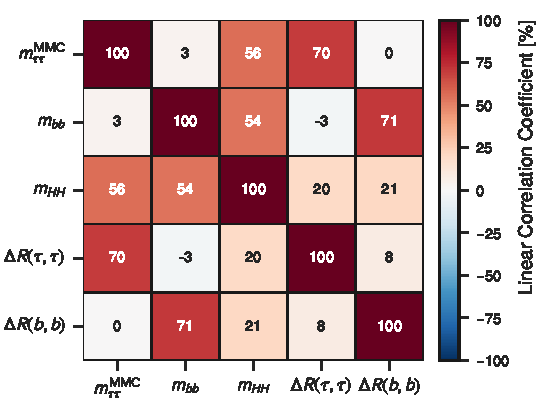
\includegraphics[width=\textwidth]{mva/correlations/Fake_pearson}
    \subcaption{Multi-jet}
  \end{subfigure}

  \caption{Correlation matrices of the MVA input variables for the SM
    \HH signal and the three largest background contributions (b) -
    (d) in the \hadhad SR.}
  \label{fig:mva_input_correlations}
  \todo[inline]{Will move to appendix (or remove completely).}
\end{figure}

%%% Local Variables:
%%% mode: latex
%%% TeX-master: "../../phd_thesis"
%%% End:
